\section{INTRODUCTION}
A central goal in robotics is the execution of long-horizon tasks in
the face of uncertainty. Readers that have spent frantic mornings
searching for lost keys understand the challenges such problems
present. Completing such a task corresponds to reasoning about
multi-modal belief distributions and obtaining a meaningful observation
can require prohibitively long sequences of primitive actions.
\begin{figure}[h]
  \centering
    \noindent
    % 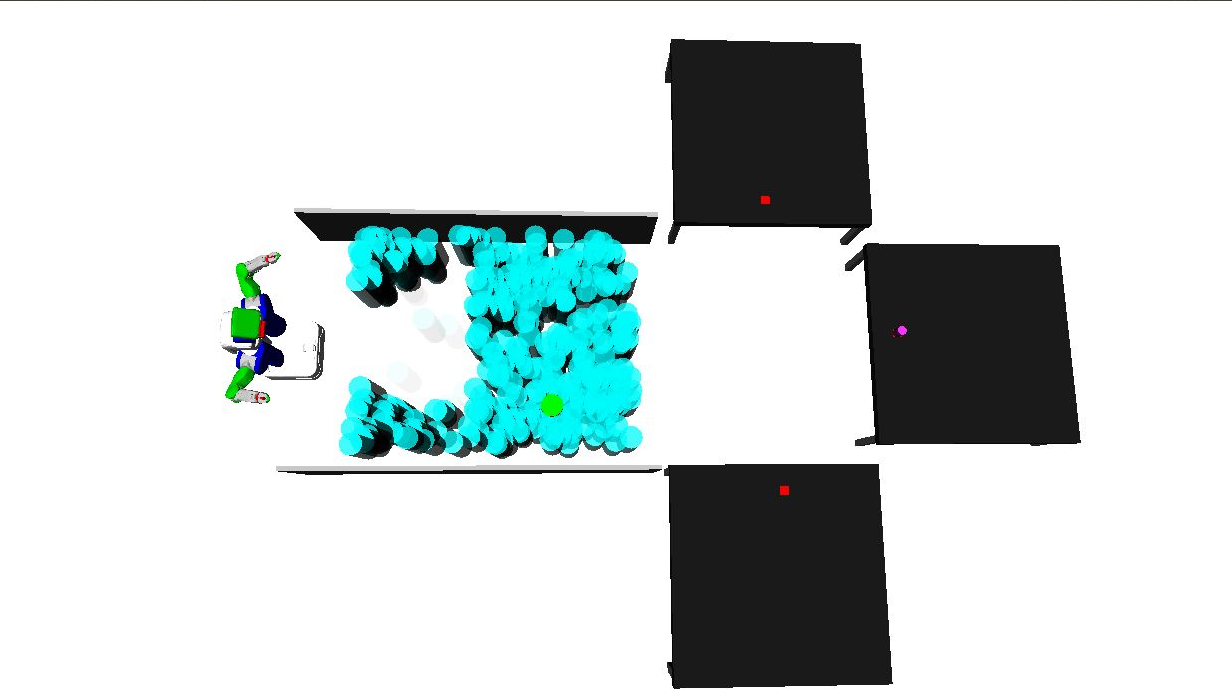
\includegraphics[width=0.45\textwidth]{corridor_images/obj_at_true_loc.png}
    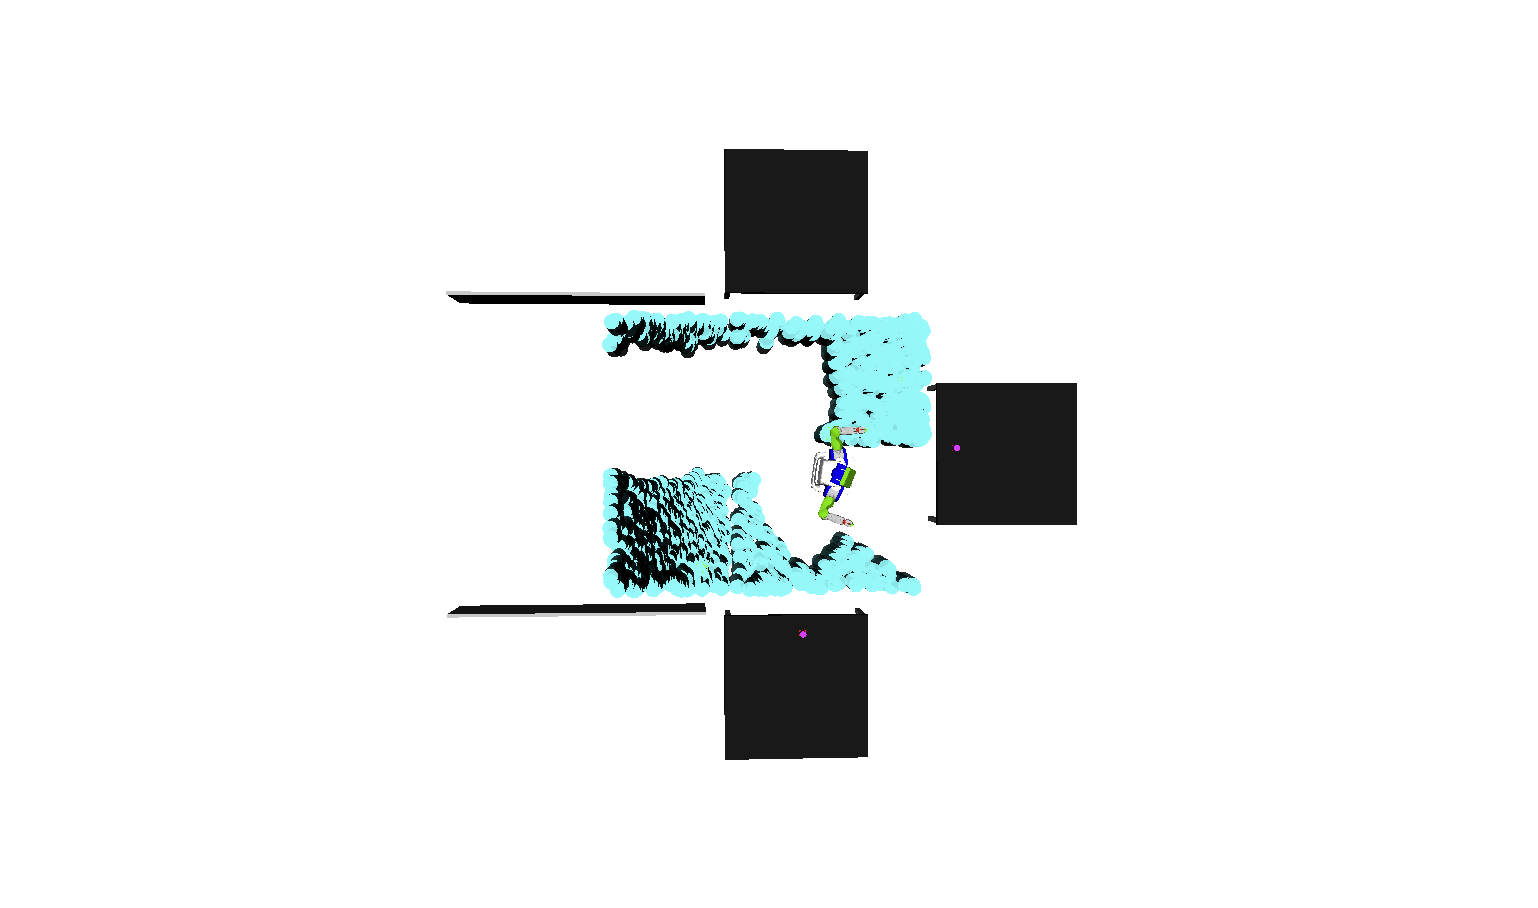
\includegraphics[trim = 160mm 90mm 0mm 90mm, clip, width=0.85\textwidth]{corridor_images/corridor_path_2.png}
  \caption{A screenshot from one of our experiments. The robot is
    tasked with navigating to the other side of the corridor through a
    uniform distribution over obstacles. Our low-level refinement
    algorithm detects likely obstructions and propagates
    this information to the high level. The objects shown are from the
    posterior distributions of multiple obstacles after several
    negative observations.}
  \label{fig:knot_steps}
\end{figure}

A solution to this task is a policy that accounts for uncertainty in
locations of objects, uncertainty in robot position, and
non-determinism in the dynamics (among other challenges). Solving such
problems exactly is far beyond the state of the art in partially
observable Markov decision processes (\pomdp).

Given the intractability of exact solution, we propose an approximate
approach. Our starting point takes inspiration from recent methods for
fully observed task and motion planning. This is a challenge in its
own right, but careful applications of abstraction, lazy
discretization, and motion planning have made
inroads~\cite{srivastava2014combined, lozano2014constraint}. These
approaches plan in an \emph{abstract} representation of a problem
(without continuous variables) then use sampling and motion planning
to \emph{refine} abstract plans into fully grounded plans with
continuous parameterizations.

An important development in approximate solutions to \pomdp s is the
\emph{maximum likelihood observation} (\mld)
determinization~\cite{platt2010belief}. This approximation assumes
that each belief state produces its maximum likelihood
observation. The result is a deterministic problem that encourages
goal directed information-gathering behavior. In this work, we extend
the domain abstraction techniques from Srivastava et
al.~\cite{srivastava2014combined} to \mld{} approximations of large
continuous \pomdp s.

Our primary contribution relies on an abstraction mechanism that
compactly represents belief state dynamics for \mld{}
determinizations. As an example, consider a fluent,
\emph{BGraspPose}(o, o\_pose\_bel, r\_pose, grasp), whose arguments
are, respectively, an object reference, a distribution over object
poses, a distribution over robot poses, and a grasp. This fluent is
true if the (unobserved) actual poses represent a successful grasp
with some preset probability. We show in \secref{sec-bsp-formulation}
that directly determinizing this formulation and applying the
skolemization approach from \cite{srivastava2014combined} leads to
unsatisfactory behavior.

Our approach avoids this issue by using properties of \mld{}
determinizations. If \emph{BGraspPose} fails to hold, then either 1)
the maximum likelihood state does not represent a successful grasp; or
2) it does, but there is too much uncertainty in the belief to have a
high probability of success. The key insight we leverage is that, in a
maximum likelihood observation determinization, the correct response
to the first scenario is to change the maximum likelihood state, while
the correct response to the second is to observe more.

We show how to use this insight to generate useful abstractions in
\secref{sec-optimism} and give a novel algorithm, Interfaced Belief
Space Planning (\ibsp), that applies a determinization-replan approach
to large continuous \pomdp s. \ibsp{} extends the interface of
\cite{srivastava2014combined} and enforces a clear separation among
extracting a plan skeleton from a domain description, refining a plan
skeleton, and determining success or failure of a plan. Our
implementation uses an off-the-shelf classical planner to generate
plan skeletons and sampling and trajectory optimization to generate
refinements and determine their validity.

An important property of our solution is that it relies on standard
belief state queries, such as sampling and maximum likelihood
computation. Such structured access to the belief state allows \ibsp{}
to work with a broad class of potentially complex state-estimation
methods with no algorithmic changes. We validate our approach in a set
of simulated partially observable mobile manipulation tasks. A
representative task is object retrieval from one of many possible
drawers. Long action sequences are required to generate useful
observations and correctly accounting for negative observations is
necessary for success. Our algorithm reasons about
obstructions and occlusions to generate plans to find its goal object,
while ensuring safety requirements are met.

%%PA: it'd be really good to include specifics about the
%%scenarios in which we evaluate our approach and specifics about the 
%% behaviors it manages to generate;   for many readers
%%interesting scenarios will make them interested in the approach,
%%lack thereof will make them wonder why they would bother reading
%%this paper...


%%PA: can we have a representative teaser figure on the first page
%%(top of the right column) ?
